\section{Présentation informelle d'un \emph{Lambda} typé}

%Les premières tentatives cherchaient à ajuster le langage \emph{Lambda} pour
%pouvoir typer l'ensemble des constructions d'OCaml. Ceci m'a permi d'acquérir
%une meilleure compréhension de l'architecture du compilateur et de l'encodage du
%langage source dans les passes intermédiaires.

\subsection{Représentation des valeurs d'OCaml}

Les extensions ont été conçues autour de la représentation des valeurs par
OCaml. Les valeurs concrètes sont :
\begin{itemize}
  \item soit des entiers, directement représenté par un scalaire,
  \item soit des blocs représentés par un pointeur vers une
zone mémoire composée d'une étiquette et d'un vecteur de valeurs.
\end{itemize}
Un bit des valeurs est réservé pour distinguer les entiers des pointeurs.

\begin{figure}
\centering
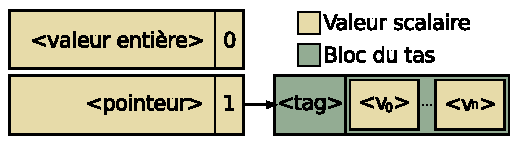
\includegraphics{media/ocaml_value}
\caption{Forme des valeurs}
\end{figure}

\paragraph{Types algébriques}

La spécificité de ML qui marque sans doute le plus ceux qui aprennent ce langage
sont les \emph{types sommes}. Les types de cette forme ont plusieurs
constructeurs de valeurs.

Ce comportement rappelle les \emph{union}s du C, mais les constructeurs des
types sommes sont disjoints : une fois construit, on peut retrouver sans
ambiguité le constructeur qui a engendré une valeur. Enfin, ces constructeurs
peuvent recevoir des paramètres. 

\begin{lstlisting}
  type address =
    | Any
    | Localhost
    | IP of int * int * int * int
    | Host of string

  let resolve addr = match addr with
    | Any -> 0, 0, 0, 0
    | Localhost -> 127, 0, 0, 1
    | IP (a,b,c,d) -> a, b, c ,d
    | Host host -> (* getaddrinfo ... *)
\end{lstlisting}

Ici, \emph{Any} est constant : il n'existe qu'une seule valeur de type
\emph{address} issue de ce constructeur. De même pour \emph{Localhost}, mais
cette unique valeur est différente de celle d'\emph{Any}. \emph{IP} et
\emph{Host} sont paramétrés.  L'analyse des constructeurs paramétrés constitue
un mécanisme sûr et vérifiable pour transporter des valeurs de différents types.

Les constructeurs constants sont encodés par des entiers, les constructeurs
paramétrés par un bloc de même arité.

La valeur des entiers et l'étiquette des blocs servent à discriminer les
différents constructeurs durant le \emph{filtrage de motif}. Les entiers
endossent ainsi le même rôle que l'étiquette des blocs; ceux-ci sont testés
dynamiquement pour choisir un branchement.

L'encodage du type \emph{address} est le suivant :
\begin{description}
  \item[Any] l'entier 0
  \item[Localhost] l'entier 1
  \item[IP] un bloc d'étiquette 0 et d'arité 4
  \item[Host] un bloc d'étiquette 1 et d'arité 1
\end{description}

La forme compilée de la fonction \emph{resolve} définie ci-dessus :

\lstset{language=Lisp}
\begin{lstlisting}
(switch* addr
   ;; Any
   case int 0: [0: 0 0 0 0]
   ;; Localhost
   case int 1: [0: 127 0 0 1]
   ;; IP
   case tag 0:
    (makeblock 0 (field 0 addr) (field 1 addr)
      (field 2 addr) (field 3 addr))
   ;; Host
   case tag 1: ...)
\end{lstlisting}
\lstset{language=Caml}

\paragraph{Variants polymorphes} 
Les variants polymorphes sont une forme plus souple de types sommes. En
particulier, ils ne nécessitent pas de déclarations préalables et peuvent
s'étendre. Dans l'analyse d'une de ces valeurs, cela se matérialise par la
présence de cas « par défaut ».

L'encodage ressemble à celui des types sommes, mais l'étiquette pour
discriminer les constructeurs paramétrés n'est plus celui du bloc. Une
indirection est ajoutée sous la forme d'un premier bloc composé de l'étiquette
et d'un pointeur vers un n-uplet contenant les paramètres.

Du point de vue du langage intermédiaire, l'étiquette devient ici une valeur de
première classe, manipulable dans le langage.  En particulier, celui-ci
peut-être testé et transformé par l'application d'opérateurs.

\begin{figure}
\centering
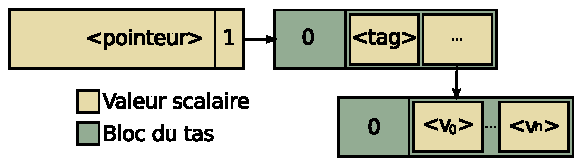
\includegraphics{media/ocaml_variant}
\caption{Forme des variants polymorphes}
\end{figure}

\subsection{Algèbre de types}

\paragraph{Système de type structurel.}
Dans OCaml, une représentation unique permet d'encoder toutes les valeurs. Il
était alors tentant de fournir des opérateurs primitifs telles que leur
composition permettent de typer toutes les valeurs. Cela forme l'essence d'un
système de type structurel.

\begin{align*}
  \syn{\tau} \tau \rightarrow \tau
    \syndesc{type flèche}
  \synor     \mu X . \tau
    \syndesc{récursion}
  \synor     \ldots
\end{align*}

Le typage des valeurs récursives est délicat avec un système structurel. Cela
conduit usuellement à une définition de la récursion dite "équirecursive" : un
type est égale à sa version développée,
  $\mu X . \tau = [X \leftarrow \mu X . \tau]$.
Malheureusement, cette formulation s'accompagne de difficulté calculatoire.

Sans surprise, seulement un sous-ensemble d'OCaml pouvait se traduire dans un
système structurel. Voici un exemple de type qui pose problème avec un tel
encodage :

\begin{lstlisting}
  type 'a tree = Leaf of 'a | Node of ('a * 'a) tree
\end{lstlisting}

La récursion non-uniforme (le paramètre $'a$ est instancié en $'a * 'a$ lors de
la récursion) nécessite la présence de fonctions au niveau des types dans sa
version structurelle, le typage devenant en général indécidable dans de telles
conditions.

\paragraph{Système de type nominal s'inspirant de System $F_c$.}
Les systèmes de type nominatifs sont la solution classique au problème
mentionné ci-dessus. 

Un nom $\epsilon$ est introduit par une définition de la forme $\epsilon
\vec{\alpha} = K \operatorname{of} \vec{\tau}$.  L'algèbre de type fait
référence à ces noms. La récursion est rendue explicite par la présence de 
constructeur $K$ qui s'interprètent comme un isomorphisme entre un nom de type
et son développement.  Cette définition de la récursion est appelée
« isorécursive ».

Le système de type d'OCaml est lui-même nominal.

\subsection{Typage sous contraintes}

La principale difficulté dans le typage de \emph{lambda} est de raffiner le
contexte en fonction des branches suivies.  Plusieurs pistes ont été suivies.

Ce type d'analyse peut se faire par une forme restreinte de typage dépendant.
Dans le typage dépendant, les valeurs peuvent intervenir dans les types. Ces
systèmes de type apporte une très grande expressivité au prix de complications
lors de la vérification des types. 

\cite{LambdaCube} propose une classification des systèmes de types dépendants en
fonction de l'ajout en expressivité au lambda-calcul simplement typé.

Nous n'introduisons ici qu'une simple dépendance entre type et identificateurs
de termes. Un système similaire a été étudié  dans \cite{Odersky02anominal} sous
le nom de "path-dependent types".

\paragraph{Types à habitant unique.}
Les types habités par une seule valeur, ou \emph{types singleton}, sont une
fonctionalité essentielle pour raffiner un type dans une branche.
Cette garantie d'unicité permet, après le test d'une valeur, de s'assurer que
son type est localement plus fin. 

Si le type était partagé par plusieurs valeurs potentiellement différente, il
serait possible d'introduire des incohérences dans le contexte.

Une fois le branchement effectué, cette information est ensuite propagée dans le
contexte par un système de contrainte.
